\documentclass{article}
\usepackage[utf8]{inputenc}
\usepackage[english]{babel}
\usepackage{mathtools}
\usepackage{graphicx}

\usepackage{multicol}
 
\addtolength{\oddsidemargin}{-1.5in}
\addtolength{\evensidemargin}{0in}
\addtolength{\textwidth}{3in}

\addtolength{\topmargin}{-.875in}
\addtolength{\textheight}{1.75in} 
 
 
\begin{document}
\begin{multicols}{3}
[
\section{NE101 Mid Term 2}
NE101 Equation Sheet, Joshua Howland, 11/3/2014]

Constants:\\
$\mu_{0} = 4 \pi \times 10 ^{-7} NA^{-2}$ or $Hm^{-1} $\\
$\epsilon = 8.854187 \times 10 ^{-12} \frac{F}{m}$\\	
$eV = 1.6022\times 10 ^{-16} J$\\
mass hydrogen $ = 1.00794u  $\\
$1u = 1.66053 \times 10^{-27} kg $\\

Shell model:\\
Intermediate Form: (unlikely on exam):\\
Magic Numbers: 2,8,20,40,58,92,112 \\

Intermediate form with spin orbit (Extreme independent shell model):\\
$1s_{1/2}^{2} 1p_{3/2}^{4} 1p_{1/2}^{2} 1d_{5/2}^{6} 2s_{1/2}^{2} 1d_{3/2}^{4} 1f_{7/2}^{8} 2p_{3/2}^{4} $\\
$1f_{5/2}^{6} 2p_{1/2}^{2} 1g_{9/2}^{10} 1g_{7/2}^{8} 2d_{5/2}^{6} 2d_{3/2}^{4}$\\
Magic Numbers: 2, 8, 20, 28, 50, 82, 126, 184\\
Notation: 1(s-0, p-1, d-2, f-3, g-4, h-5)\\

Example: Give the expected shell-model spin and parity assignments for the ground states of: (a) $ \prescript{7}{}{Li} $: 3p, 4n: 1 unpaired proton.  Proton shells are: $1s_{1/2}^{2}1p_{3/2}^{1}$.  $\ell = 1 (p=1)$, $\pi = -$, $J_{\pi} = \frac{3}{2}^{-}$ (b) $ \prescript{11}{}{B} $: 5p, 6n: 1 unpaired proton.  Proton shells are: $1s_{1/2}^{2}1p_{3/2}^{3}$.  $\ell = 1 (p=1)$, $\pi = -$, $J_{\pi} = \frac{3}{2}^{-}$ (c) $ \prescript{15}{}{B} $: 6p, 9n: 1 unpaired neutron.  Neutron shells are: $1s_{1/2}^{2}1p_{3/2}^{4}1p_{1/2}^{2}1d_{5/2}^{1}$.  $\ell = 2(d=2)$, $\pi = +$, $J_{\pi} = \frac{5}{2}^{+}$ Note: $\prescript{15}{}{C}$ prediction wrong, observed value is $\frac{1}{2}^{+}$\\
For odd-odd nuclei: $\vec{I} = \vec{j}_{p} + \vec{j}_{n}$\\
In ground state, $\vec{s}_{p}$ and $\vec{s}_{n}$ are parallel\\
$j_{p} = \ell_{p} + s_{p}$ and $j_{n} = \ell_{n} + s_{n}$\\
Note: $\ell$ and $s$ not always parallel!\\
To calculate $J_{\pi}$, match $\ell$ to correct orbital for p and n, with spins parallel and add parities!\\

Example: Calculate $I^{\pi}$ assignments of: (a) $ \prescript{26}{}{Na} $: 11p, 15n.  p: $1d_{5/2}^{3}$, $\ell = 2$, $2 + \frac{1}{2} = \frac{5}{2}$. n: $2s_{1/2}^{1}$, $\ell = 0$, $0 + \frac{1}{2} = \frac{1}{2	}$.  Total $J^{\pi} = 3^{+}$ (b)  $ \prescript{28}{}{Na} $: 11p, 17n.  p: $1d_{5/2}^{3}$, $\ell = 2$, $2 + \frac{1}{2} = \frac{5}{2}$. n: $1d_{3/2}^{1}$, $\ell = 2$, $-2 + \frac{1}{2} = |-\frac{1}{2}|$.  Total $J^{\pi} = 1^{+}$ \\
Shell model predicts that even-even nuclei will have a spin of $0^{+}$

Unit of EM energy called photon.  "Quantum" of vibrational energy called phonon\\
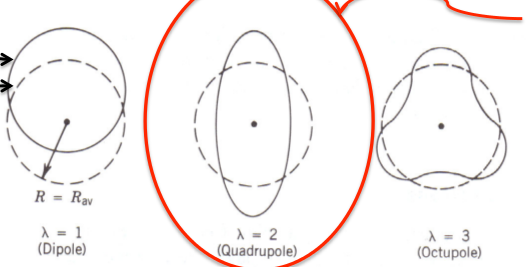
\includegraphics[width=4cm]{images/vibrations.jpg}\\
Vibrational model best for even-even nuclei with A<150?(methinks)\\
Energy of vibration: $E = hv$, v = frequency in $\frac{vibrations}{sec}$
Magnetic moments for first $2^{+}$ states predicted to be $2(\frac{Z}{A})$ and $\frac{E(2^{+})}{E(4^{+})}$ is predicted to $=2$ \\
Example:  Compute vibrational frequency associated with typical quadrupole vibrations, then compare typical lifetimes of $2^{+}$ excited states in vibrational nuclei to their vibrational frequency:  $\prescript{120}{}{Te}$ is a good choice (even-even, A<150), low lying excited state at $2^{+}$.  $E = hv$, $v = \frac{E}{h} = \frac{0.5604Mev}{4.135\times10^{-21}\frac{Mev}{s}} = 1.355\times10^{20}\frac{1}{sec}$.  T is much shorter than half life, so vibrates many times before decaying. $<\alpha>$ goes to 0, so we cant observe anything based on it, however $<\alpha^{2}>$ does not!

Nuclear Rotations:  Can only be observed in nuclei with non-spherical equilibrium shapes\\
$R(\theta,\phi) = R_{av}[1+\beta Y_{20}(\theta,\phi)]$\\
$\beta = \frac{4}{3} \sqrt{\frac{\pi}{5}} \frac{\Delta R}{R_{av}}$, $R_{av} = R_{0}A^{\frac{1}{3}}$\\
$E = \frac{\hbar^{2}}{2\Im}J(J+1)$, $\Im$= moment of inertia\\
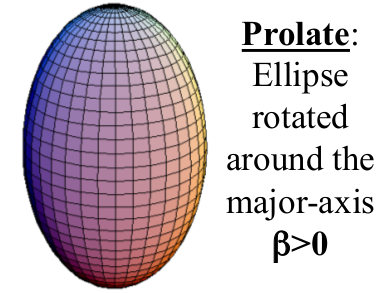
\includegraphics[width=3cm]{images/prolate.png}
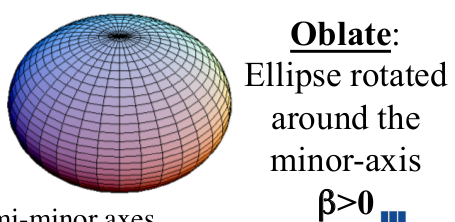
\includegraphics[width=3cm]{images/oblate.png}\\
$P = \frac{N_{p}^{valence}N_{n}^{valence}}{N_{p}^{valence}+N_{n}^{valence}}$, $P>4$ deformed\\
If the nucleus was rigid: $\Im_{rigid} = \frac{2}{5}MR_{av}^{2}(1+0.31\beta) \approx 6 kev$ for A = 170, but the observed value is 15Kev, so rotation is non rigid.  $\omega_{rotation} \approx 10^{20} \frac{rad}{sec} \approx 0.002c$ on surface.  Nuclear rotation is much slower than motion of nucleons, thus it is a type of collective motion. Deformation lowers energies of states moving inside the nucleus, raises energies of states spending more time outside nucleus\\??Add backbending/nisson model??\\
Collective model magnetic moment: 
$\mu (I) = I \frac{Z}{A} \mu_{N}$\\

Alpha Decay: First type of decay discovered, least penetrating, emitted almost entirely by large nuclei, p conserved\\
 $(Z,A)\rightarrow(Z-2,A-4) + \prescript{4}{2}{He}_{2}$\\
 $Q_{\alpha} = M(Z,A)c^{2} - M_{product}c^{2} - M(\prescript{4}{2}{He}_{2})$\\
 $Q_{\alpha} = K.E.(Z-2,A-4) + K.E.(\prescript{4}{2}{He}_{2})$\\
 $K.E. = T = \frac{p^{2}}{2m}$\\
 $Q = T_{\alpha} + T_{Z-2,A-4} = T_{\alpha} + \frac{p^2}{2M_{Z-2,A-4}}$\\
 $Q = T_{\alpha} + T_{\alpha}(\frac{M_{\alpha}}{M_{Z-2,A-4}})$\\
 $T_{\alpha} = \frac{Q}{1 + \frac{M_{\alpha}}{M_{Z-2,A-4}}} = \frac{Q}{1 + \frac{4}{A}}$\\
 $T_{x^{\prime}} = \frac{Q}{1 + \frac{m_{x^{\prime}}}{m_{\alpha}}}$\\
Example: $Q_{\alpha} = [M(\prescript{235}{}{U}) - M(\prescript{231}{}{Th}) - M(\alpha)]c^{2} = 4.678 Mev$.  $T_{\alpha} = 4.678Mev(1-\frac{4}{235}) = 4.598 Mev$, $T_{\prescript{231}{}{Th}} = Q_{\alpha} - T_{\alpha} = (4.678 - 4.598)Mev = 0.080Mev$\\
Majority of $\prescript{4}{}{He}$ on earth comes from $\alpha$ decay of U,Th and their daughters\\
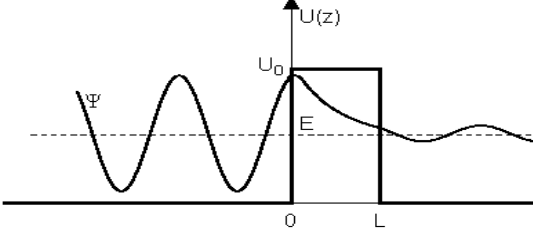
\includegraphics[width=3cm]{images/alpha_barrier.png} Barrier Penetration\\
$T = \frac{1}{1 + \frac{1}{4}\frac{U_{0}^{2}}{E(U_{0}-E)}sinh^{2}(\alpha L)}$\\
$\alpha = \sqrt{\frac{2m_{\alpha}E_{\alpha}}{\hbar^{2}}} \approx 17.5 fm$,  $T\approx10^{-29}$\\
BAD.  Instead, break up barrier into smaller chunks\\
$P \approx e^{-2\alpha a} = exp(-2\sqrt{\frac{2m_{\alpha}\frac{1}{2}(B-Q)}{\hbar^{2}}}x\frac{1}{2}(b-a))$\\
Angular Momentum in Alpha Decay: Any angular momentum carried away by the $\alpha$-particle is purely orbital\\
Parity change = $(-1)^{\ell_{\alpha}}$.  If the initial and final parities are the same, $\ell$ is even.  If they are different, $\ell$ is odd.  For a given $\alpha$ energy Q, the probability of barrier penetration decreases with increasing $\ell$\\
Example: $\prescript{235}{}{U}$ decay:\\
 $\frac{\ell(\ell+1)}{2mr^{2}} = \frac{\ell(\ell+1)(197.3Mev f`m)^{2}}{2(4)(931.5Mev)(7.4fm)^{2}}$,\\ $\ell(\ell+1)x0.087Mev \rightarrow 0.174MeV$ for $\ell = 1$\\
 Alpha particle spectroscopy: 1. Make source of $\alpha$-decaying nuclei.  Must be thin for $\alpha$'s to escape without losing much energy.  2. Measure the number of $\alpha$'s as a function of their energies.  You can also measure g-rays emitted from excited states populated by $\alpha$ decay.\\

Copy hw 5 problems 8 and 10!!!\\


\end{multicols}
 
\end{document}